\chapter{Distribuzioni}

\section{Stimare la Distribuzione}\label{stimare-distribuzione}

Per stimare una distribuzione avendo solo i dati iniziali del problema effettua
le seguenti operazioni:


\paragraph{N.B.} \textit{nel caso di Intervalli,} $\text{categoria}_i$ \textit{va sostituito con}
$\text{Punto Medio Intervallo}_i$

\begin{enumerate}
      \item $n = \sum{f_i}$: assicurati di aver calcolato la somma totale delle
            osservazioni
      \item Calcola la \textbf{Media}: \begin{enumerate}
                  \item Aggiungi \textit{Colonna Totale}: $\text{categoria}_i * f_i$
                  \item Calcola la media effettiva con: $media = \frac{\sum
                                    totale}{n}$
            \end{enumerate}
      \item Calcola la \textbf{Varianza $\sigma^2$}: \begin{enumerate}
                  \item Aggiungi \textit{Colonna ris}: $(\text{categoria}_i -
                              \text{media})^2 * f_i$
                  \item Calcola la varianza effettiva con: $\sigma^2 = \frac{\sum
                                    \text{ris}}{n -1}$
            \end{enumerate}
      \item Calcola la \textbf{Deviazione Standard $\sigma$}: \begin{enumerate}
                  \item $\sigma = \sqrt{\sigma^2}$
            \end{enumerate}
      \item Calcola $V = \frac{\sigma}{\text{media}}$
\end{enumerate}

Una volta completati tutti i calcoli controlla se il coefficiente $V$ è vicino
ad 1 e:
\begin{itemize}
      \item \textbf{se lo è} allora utilizza l'\textbf{Esponenziale},
      \item \textbf{se non lo è} è \textbf{Poissoniana} ma per avere una verifica,
            controlla che la media e la varianza siano uguali.
\end{itemize}

\paragraph{Note:}\ \\
Si può avere una prima idea del tipo di distribuzione anche
osservando le frequenze per categoria:
\begin{itemize}
      \item Se le frequenze hanno valori alti per le prime categorie e poi
            decrescono, probabilmente è esponenziale negativa.
      \item Se le frequenze hanno valori bassi per le prime categorie e poi
            crescono, probabilmente è esponenziale\dots
      \item Se le frequenze hanno valori alti nelle categorie centrali e bassi
            verso le categorie agli estremi, probabilmente è Poissoniana
      \item Nel caso in cui sia geometrica solitamente viene esplicitato.
\end{itemize}

\section{Calcolare la Probabilità di una Distribuzione} \label{pi}

\paragraph{N.B.} \textit{nel caso di Intervalli,} $\text{categoria}_i$ \textit{va sostituito con}
$\text{intervallo}_i$

\subsection{Esponenziale}

\textit{Numero di Parametri:} 1

\subsubsection{Senza Intervalli}

\[
      p(i) = \frac{e^{\frac{- \text{categoria}_i}{\text{media}}}}{\text{media}}
\]

\subsubsection{Con Intervalli}

\[
      p(i) = 1 - e^{\frac{- \text{intervallo}_i}{\text{media}}}
\]

\subsection{Poisson}

\textit{Numero di Parametri:} 1

\[
      p(i) = \frac{e^{- \text{media}} * \text{media}^{\text{categoria}_i}}{\text{categoria}_i !}
\]

\subsection{Geometrica}

\textit{Numero di Parametri:} 1

\[
      p(i) = \rho * (1 - \rho)^{\text{categoria}_i}
\]

\subsection{Normale}

\textit{Numero di Parametri:} 2

\subsection{Uniforme}

\textit{Numero di Parametri:} 0

\[
      p(i) = 1 / \text{numero categorie}
\]

\section{Come Raggruppare} \label{raggruppare}

Raggruppare le categorie se $\exists \ categoria < 5$:
\begin{itemize}
      \item Parti dall'ultimo a salire (dal basso verso l'alto delle
            categorie)
      \item Raggruppale tutte nell'ultima categoria che le faccia
            diventare maggiori di 5 sommando le frequenze.
      \item \textit{Esempio}:
            \begin{figure}[H]
                  \centering
                  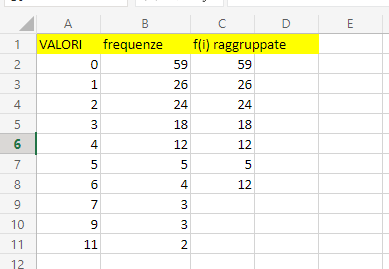
\includegraphics[width=6cm, keepaspectratio]{capitoli/goodnes_of_fit/imgs/vesceragay.png}
                  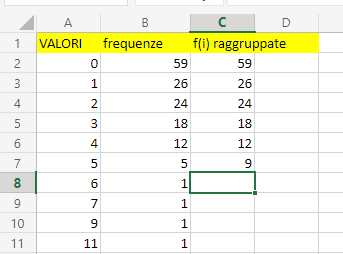
\includegraphics[width=5.5cm, keepaspectratio]{capitoli/goodnes_of_fit/imgs/POSTAMOLTOGAY.png}
            \end{figure}
\end{itemize}